\section{Introduction}
\label{secall:intro}
\subsection{Physics motivation}
\label{subsecall:motivation}
\subsection{LHC heavy-ion running}
\label{subsecall:running}

\begin{figure}[!htb]
\begin{center}
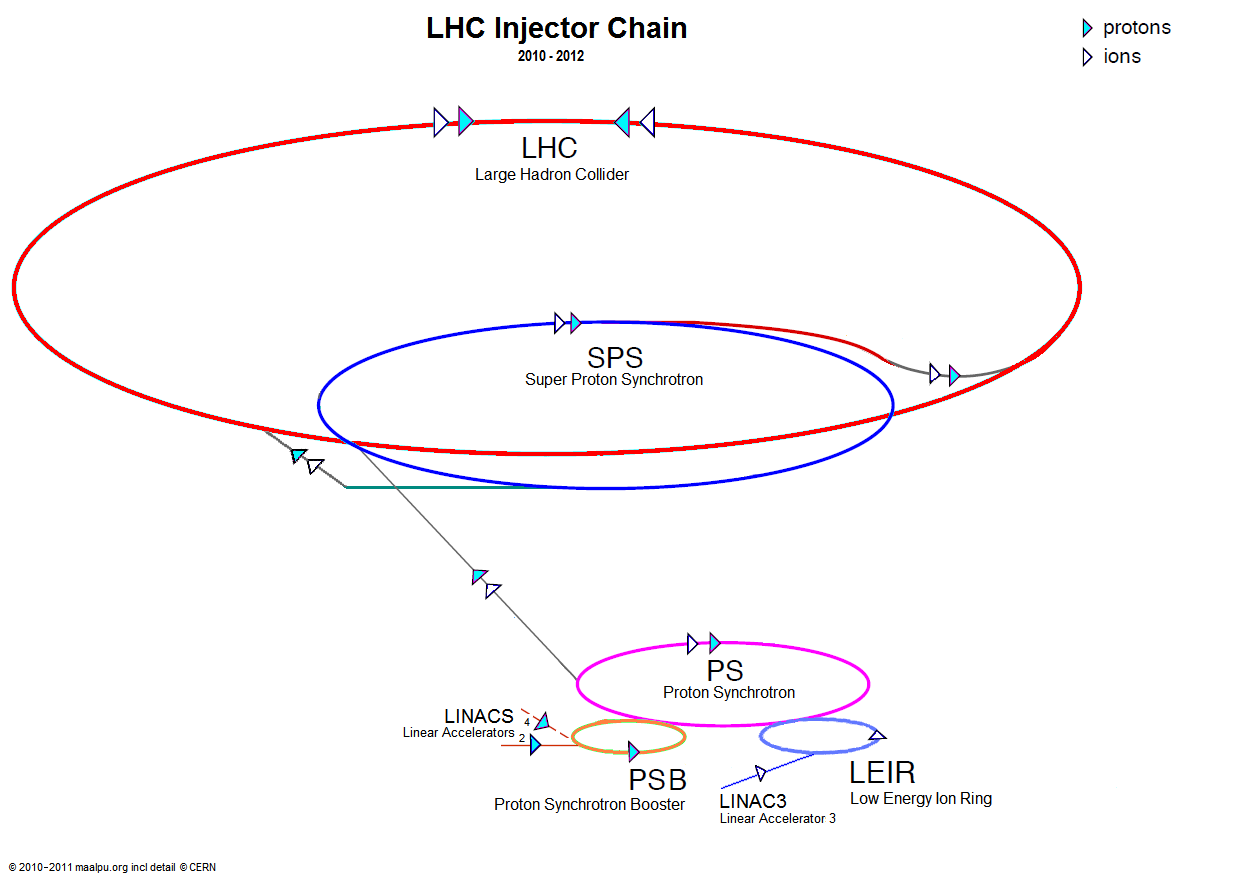
\includegraphics[width=0.8\textwidth]{introduction_figs/LHC_chain.png}
\caption[]{Schematic view of LHC injector chain, showing the path of both protons and ions.}
\label{fig:pas:intro:lhc}
\end{center}
\end{figure}

Heavy ion running at the Large Hadron Collider had been planned long before the machine was built.
This was based on the interest in the physics at the CERN SPS, which was colliding light ions since
1986 and heavy ions since 1994, and as a natural extension to the already-planned program
at the Relativistic Heavy Ion Collider (RHIC).
The accelerator complex is shown in Figure~\ref{fig:pas:intro:lhc}.
Ions start their path to collisions at the ECR (electron cyclotron resonance) ion source,
which provides lead ions stripped to values around Pb$^{29+}$, which are passed through
a spectrometer to select Pb$^{29+}$ and accelerated in a linear accelerator to 4.2 MeV/n.
They are then stripped to around Pb$^{54+}$ by a 0.3 $\mu$m carbon foil and the
Pb$^{54+}$ are selected by a spectrometer to be fed into the CERN Low Energy Ion Ring (LEIR).
LEIR is used to transform a set of low intensity ion pulses from the LINAC into shorter
bunches with higher intensity.  This is done by filling the available phase space in
three dimensions.  After this, electron cooling is applied to shrink the beam to increase the
bunch density, and decelerate it into ``a stack sitting slightly inside the central orbit''.
At this point, seven pulses are captured, split into two bunches, and then accelerated to
72 MeV/n.
The bunches from LEIR are then sent to the CERN PS (Proton Synchrotron), accelerated to
5.9 GeV/n and stripped fully to Pb$^{82+}$ using a 0.8 mm aluminium foil.  These ions
are then sent to the SPS where they are acceleated to 177 GeV/n and injected into the LHC.

To date, there have been three heavy ion runs at the LHC.
The first run was in November/December 2010, 
which provided 120 colliding bunches of lead ions in each ring, with a center of mass energy per nucleon
pair of $\energy =2.76$ TeV, a peak luminosity of $3 \times 10^{25} / \mathrm{cm}^2 s$ and an integrated luminosity
of 7 $\mu \mathrm{b}^{-1}$, corresponding to about 50 million minimum bias events.
The second run was in November/December 2011, which provided about 360 colliding bunches of lead ions per ring, 
also at $\energy =2.76$ TeV, a peak luminosity of 
about $5 \times 10^{26}  / \mathrm{cm}^2 s$ and an integrated luminosity of
about 150 $\mu \mathrm{b}^{-1}$, a factor of 20 increase over 2010.
The third run, in January/February 2013, provided proton-lead collisions
at $\energy=5.02$ TeV but these results are not discussed
in detail in this review.

\subsection{Detectors at the LHC}
\label{subsecall:detectors}

\subsubsection{ATLAS}

\begin{figure}[!htb]
\begin{center}
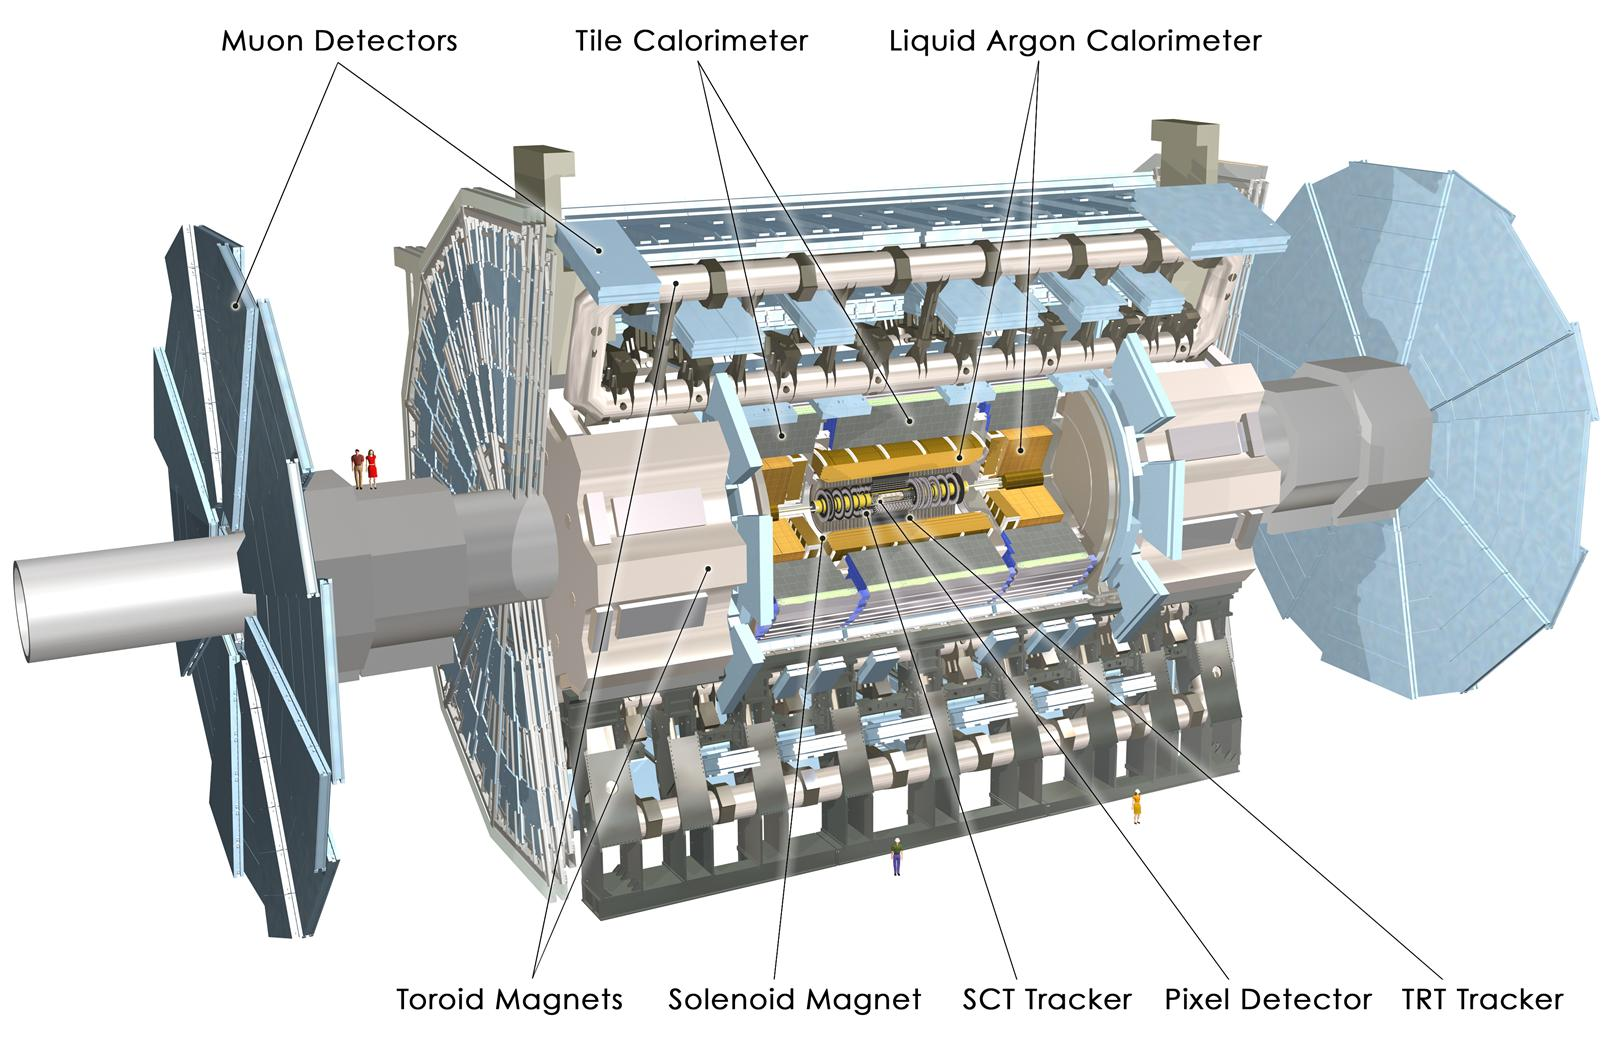
\includegraphics[height=0.49\textwidth]{introduction_figs/0803012_05-A4-at-144-dpi.jpg}
\caption[]{Schematic view of ATLAS detector at the LHC, highlighting the major subsystems.}
\label{fig:pas:intro:atlas}
\end{center}
\end{figure}

%ATLAS
The ATLAS detector, shown in Figure~\ref{fig:pas:intro:atlas} is one of the general-purpose particle physics
detectors at the LHC.  
It has three main detector systems: the inner detector (ID), the calorimeter,
and the muon spectrometer (MS).
%
The inner detector tracks charged particles using three separate detector
technologies, and the spectrometer is immersed in a 2T axial field from a 
superconducting solenoid magnet 1.2m from the nominal beam axis.
The pixel detector typically provides three high-resolution space points
with three layers of pixel detector surrounding the beam pipe within
$|z|<400 mm$ (covering approximately $|\eta|<2$ and 4 disks at forward
angles covering out to $|\eta|<2.5$.
The semiconductor tracker detectors are silicon strips covering out to
$|\eta|<X$ in the barrel region and $|\eta|<2.5$ in the forward regions.
The transition-radiation tracker covers $|\eta|<2$ with straw tubes in
both the barrel and forward regions.
%
The ATLAS calorimeter has large coverage in pseudorapidity ($|\eta|<4.9$)
and longitudinal segmentation in both electromagnetic and hadronic
sections.
In the barrel region, the electromagnetic calorimeter has three
layers and a presampler layer, all using liquid argon technology.  
The first layer has very high resolution
in the $\eta$ direction, allowing discrimination of photons from
neutral hadron decays.
The second layer is coarser but deeper, providing the primary energy
measurement for electromagnetically interacting particles (photons and
electrons), while the third layer is there to catch the tails of the
deposited electromagnetic showers.
%
The ATLAS hadronic calorimeter uses steel absorber and measures the
hadronic showers by means of scintillating tiles.
In the endcap region, beyond $|\eta|=2$, 
both hadronic and electromagnetic sections use LAr technology with
relativly coarse cell segmentation.
The ATLAS forward calorimeter (FCal) covers $|\eta|=3.2-4.9$, using
a matrix of copper and liquid argon in the electromagnetic section,
and tungsten and liquid argon for the hadronic section.
%
The ATLAS muon spectrometer covers $|\eta|<2.7$ with precision drift
chambers
in the barrel region and cathode strip chambers in the forward region.
The bending of muons is provided by three air-core toroids, giving
a momentum resolution ranging from approximately 2\% up to about
10\% at $\pT=1$ TeV.
%

ATLAS provides a sophisticated multi-level trigger system for 
selection of physics objects (jets, taus, photons, electrons, muons,
and missing transverse energy).
Jet triggering is done both seeding on energy deposited into localized
regions of the calorimeter, as well as a full reconstruction of the jets
using a similar algorithm as used in the offline analysis.
Electron and photon triggering uses smaller regions in the calorimeter
than for jets, and also applies selections based on the measured shower
shape and leakage in the hadronic sections.
Muon triggering is provided by thin-gap chambers and resistive plate chambers,
covering about 90\% of the solid angle out to $|\eta|=2.7$.
In general, triggering on tau leptons and missing transverse energy (e.g.
from $W$ bosons) is not utilized for any heavy ion analysis, as both
are highly contaminated by the large fluctuations in the 
underlying event.
